\documentclass[12pt]{ctexart}

\usepackage[a4paper,margin=2.5cm]{geometry}
\usepackage{setspace}
\usepackage{titlesec}
\usepackage{xcolor}
\usepackage{indentfirst}
\usepackage{float}
\usepackage{graphicx}
\usepackage{float}
\usepackage{tikz}
\usetikzlibrary{arrows.meta,positioning}
\usepackage{graphicx}

\usetikzlibrary{arrows.meta}
\usetikzlibrary{arrows.meta,positioning}

\setlength{\parindent}{0em}
\setstretch{1.5}

% 标题格式
\titleformat{\section}{\bfseries\zihao{4}}{}{0em}{}
\titleformat{\subsection}{\bfseries\zihao{-4}}{}{0em}{}

% 自定义空行
\newcommand{\blankline}{\vspace{1.5em}}

\begin{document}

\begin{figure}[H]
    \centering
    
\includegraphics[width=0.70\textwidth]{img/0.png}
\end{figure}
% 首页不显示页码
\thispagestyle{empty}


{\heiti\zihao{4} 一、实验名称：}
\textbf{Radius协议综合实验}


{\heiti\zihao{4} 二、实验学时：4}


{\heiti\zihao{4} 三、实验内容和目的：}

本实验基于 Windows Server 搭建 Radius 综合实验环境，完成域控制器、DNS、DHCP、VPN 服务器以及 RADIUS 服务器的配置，实现远程客户端通过 VPN 接入内部网络，并由 RADIUS 服务器完成用户认证与授权。实验最后通过端口扫描程序对目标主机的相关服务端口进行测试，验证各项服务是否正常开启。

通过本实验，掌握 RADIUS 协议的基本原理及其在远程接入中的应用方式，理解 VPN 与 RADIUS、DHCP、DNS 等服务之间的协同工作过程，熟悉 Windows Server 环境下相关网络服务的配置方法，并提高对网络安全系统综合部署、调试和分析问题的能力。


{\heiti\zihao{4} 四、实验原理：}

RADIUS是一种常见的远程接入认证协议，主要用于实现 AAA 功能，即认证、授权和计费。它通常应用于 VPN、无线接入和拨号接入等场景中，可以将用户身份验证与访问控制集中到认证服务器统一完成，提高网络管理效率和安全性。

在本实验中，远程客户端首先向 VPN 服务器发起连接请求，VPN 服务器作为 RADIUS 客户端，将用户提交的用户名和密码等认证信息发送给 RADIUS 服务器。RADIUS 服务器根据活动目录中的用户信息以及预先配置好的远程访问策略，对用户进行身份认证与访问授权。若认证成功，VPN 服务器则允许客户端建立连接，并为其分配内部网络地址，使客户端能够访问内部资源；若认证失败，则拒绝用户接入。

RADIUS 协议基于 UDP 传输，其中认证和授权通常使用 1812 端口，计费通常使用 1813 端口。由于 RADIUS 采用客户端/服务器结构，因此 VPN 服务器与 RADIUS 服务器之间需要预先配置共享密钥，用于保证双方通信的合法性和一致性。如果共享密钥不一致、客户端地址配置错误或用户没有远程访问权限，都会导致认证失败。

为了使整个实验系统正常运行，还需要其他网络服务进行配合。其中，域控制器用于统一管理用户账号和访问权限；DNS 服务器用于域名解析，保证域环境正常运行；DHCP 服务器用于在客户端成功接入后动态分配内部 IP 地址；VPN 服务器则负责建立远程接入通道。通过这些服务的协同工作，可以构建一个较完整的远程访问认证环境。

此外，网络服务最终都依赖传输层端口对外提供功能，因此实验中还通过编写端口扫描程序，对目标主机的指定端口进行连接测试。若端口连接成功，则说明对应服务处于开启状态；若连接失败，则说明该端口未开放或服务未正常运行。通过端口扫描测试，可以进一步验证所配置服务器的网络服务状态。

\begin{table}[H]
\centering
\caption{实验中主要服务及作用}
\begin{tabular}{|c|p{9cm}|}
\hline
\textbf{服务} & \textbf{作用} \\ \hline
域控制器 & 统一管理用户账号、用户权限以及相关安全策略 \\ \hline
DNS 服务器 & 提供域名解析服务，保证域环境及网络服务正常运行 \\ \hline
DHCP 服务器 & 为成功接入 VPN 的客户端动态分配内部网络地址 \\ \hline
VPN 服务器 & 接收远程客户端的连接请求，建立安全接入通道 \\ \hline
RADIUS 服务器 & 对用户进行认证、授权和计费管理 \\ \hline
端口扫描程序 & 检测目标主机端口开放情况，验证网络服务是否正常启动 \\ \hline
\end{tabular}
\end{table}

\begin{figure}[H]
\centering
\begin{tikzpicture}[
    x=1cm,y=1cm,
    >=Stealth,
    font=\small,
    box/.style={
        draw,
        minimum width=3.4cm,
        minimum height=1.0cm,
        align=center
    }
]

\node[box] (client) at (0,0) {远程客户端};
\node[box] (vpn)    at (5.5,0) {VPN服务器\\（RADIUS客户端）};
\node[box] (radius) at (11,0) {RADIUS服务器};

\node[box] (dhcp) at (5.5,-3) {DHCP服务器};
\node[box] (dc)   at (11,-3) {域控制器/DNS};

\draw[->] (client.east) -- (vpn.west)
    node[midway, above=6pt] {VPN请求};

\draw[->] (vpn.east) -- (radius.west)
    node[midway, above=6pt] {认证请求};

\draw[->] (radius.west) -- ++(-1.7,0)
    node[midway, below=6pt] {认证结果};

\draw[->] (dhcp.north) -- (vpn.south)
    node[midway, left=8pt] {分配内部IP};

\draw[->] (dc.north) -- (radius.south)
    node[midway, right=8pt] {用户信息/策略};

\end{tikzpicture}
\caption{RADIUS认证与VPN接入原理图}
\end{figure}


{\heiti\zihao{4} 五、实验器材（设备、元器件）：}

\begin{enumerate}
    \item 安装虚拟机软件的计算机一台；
    \item Windows Server 虚拟机一台；
    \item Windows 客户端虚拟机一台；
    \item 桥接网络和 Host-Only 网络环境；
    \item Windows Server 自带的 DNS、DHCP、VPN、RADIUS 等服务组件；
    \item 编写端口扫描程序所需的编程环境。
\end{enumerate}


{\heiti\zihao{4} 六、实验步骤：}

\begin{enumerate}
\item 升级Windows Server为域控制器
\item 配置DNS服务器
\item 配置DHCP服务器
\item 配置Internet验证服务,并创建Radius客户端和远程访问策略
\item 配置VPN服务器
\item 配置远程客户端
\item 测试客户端连接
\end{enumerate}




{\heiti\zihao{4} 七、实验数据及结果分析：}

\subsection*{1. 升级Windows Server为域控制器}

在搭建域环境之前，首先需要完成服务器实验环境和网络基础配置。实验中为 Windows Server 2022 虚拟机分配了 2\,GB 内存、2 个处理器核心和 60\,GB 硬盘空间，并为其添加两块网络适配器，分别用于外部网络和内部网络。其中，外网网卡用于后续 VPN 远程接入，内网网卡用于域环境内部通信。服务器的虚拟机硬件配置和双网卡配置如下所示。

\begin{figure}[H]
    \centering
    \begin{minipage}{0.48\textwidth}
        \centering
        
\includegraphics[width=\textwidth]{img/1.png}
    \end{minipage}
    \hfill
    \begin{minipage}{0.48\textwidth}
        \centering
        
\includegraphics[width=\textwidth]{img/2.png}
    \end{minipage}
    \caption{域控制器部署前的实验环境配置}
\end{figure}

完成双网卡添加后，需要分别对网卡进行命名和参数设置。实验中将两块网卡分别命名为“外网”和“内网”，其中内网网卡设置为固定地址 \texttt{192.168.162.10/24}，DNS 服务器指向本机；随后通过 \texttt{ipconfig /all} 对服务器网络参数进行检查，确认外网与内网地址配置正确，为后续域控安装提供网络基础。相关配置过程如下所示。

\begin{figure}[H]
    \centering
    \begin{minipage}{0.48\textwidth}
        \centering
        
\includegraphics[width=\textwidth]{img/3.png}
    \end{minipage}
    \hfill
    \begin{minipage}{0.48\textwidth}
        \centering
        
\includegraphics[width=\textwidth]{img/4.png}
    \end{minipage}
    \caption{服务器网络基础配置}
\end{figure}

\begin{figure}[H]
    \centering
    
\includegraphics[width=0.72\textwidth]{img/5.png}
    \caption{在服务器管理器中添加 Active Directory 域服务角色}
\end{figure}

在服务器管理器中添加 \texttt{Active Directory 域服务} 角色后，继续执行“将此服务器提升为域控制器”。实验中选择“添加新林”，并将根域名设置为 \texttt{radius.local}；随后在域控制器选项中勾选 DNS 服务器和全局编录，并设置目录服务还原模式密码。安装过程中系统会自动完成相关组件部署，安装完成后服务器重启并正式加入域环境。该过程如下所示。

\begin{figure}[H]
    \centering
    \begin{minipage}{0.48\textwidth}
        \centering
        
\includegraphics[width=\textwidth]{img/6.png}
    \end{minipage}
    \hfill
    \begin{minipage}{0.48\textwidth}
        \centering
        
\includegraphics[width=\textwidth]{img/7.png}
    \end{minipage}

    \vspace{0.6em}

    \begin{minipage}{0.48\textwidth}
        \centering
        
\includegraphics[width=\textwidth]{img/8.png}
    \end{minipage}
    \hfill
    \begin{minipage}{0.48\textwidth}
        \centering
        
\includegraphics[width=\textwidth]{img/9.png}
    \end{minipage}
    \caption{域控制器提升与安装过程}
\end{figure}

域控制器配置完成后，可以在系统中看到服务器已经加入 \texttt{radius.local} 域，并能够正常打开“Active Directory 用户和计算机”管理界面。这说明 Windows Server 已成功升级为域控制器，为后续创建域用户、配置 DNS、DHCP、RADIUS 和 VPN 服务提供了基础环境。验证结果如下所示。

\begin{figure}[H]
    \centering
    \begin{minipage}{0.48\textwidth}
        \centering
        
\includegraphics[width=\textwidth]{img/10.png}
    \end{minipage}
    \hfill
    \begin{minipage}{0.48\textwidth}
        \centering
        
\includegraphics[width=\textwidth]{img/11.png}
    \end{minipage}
    \caption{域控制器安装完成后的验证结果}
\end{figure}


\subsection*{2. 配置DNS服务器}

在将 Windows Server 2022 成功提升为域控制器后，系统已自动安装 DNS 服务。为了保证后续域用户认证、RADIUS 身份验证以及 VPN 远程接入能够正常进行，还需要对 DNS 服务器进行进一步检查与配置。本实验中，服务器内网地址为 \texttt{192.168.162.10}，域名为 \texttt{radius.local}，因此 DNS 服务的配置重点包括：检查本机 DNS 参数、创建主机记录、建立反向查找区域，并通过正向和反向解析测试验证配置结果。

首先，通过 \texttt{ipconfig /all} 检查服务器网络参数，确认服务器当前的 DNS 服务器已指向本机回环地址，从而保证域控制器能够调用本地 DNS 服务完成名称解析。相关结果如图所示。

\begin{figure}[H]
    \centering
    
\includegraphics[width=0.72\textwidth]{img/18.png}
    \caption{通过 \texttt{ipconfig /all} 检查服务器 DNS 参数}
\end{figure}

随后打开 DNS 管理器，在正向查找区域中查看 \texttt{radius.local} 区域。为了便于后续测试，在该区域中新建主机记录，将主机名 \texttt{server} 映射到服务器内网地址 \texttt{192.168.162.10}，并同时勾选创建对应的 PTR 记录。配置完成后，可以在 \texttt{radius.local} 区域中看到相应的主机记录。相关过程如图所示。

\begin{figure}[H]
    \centering
    \begin{minipage}{0.48\textwidth}
        \centering
        
\includegraphics[width=\textwidth]{img/15.png}
    \end{minipage}
    \hfill
    \begin{minipage}{0.48\textwidth}
        \centering
        
\includegraphics[width=\textwidth]{img/14.png}
    \end{minipage}
    \caption{在正向查找区域中添加主机记录并查看 DNS 记录}
\end{figure}

为了实现 IP 地址到主机名的反向解析，还需要建立反向查找区域。实验中根据服务器内网网段 \texttt{192.168.162.0/24}，在 DNS 管理器中新建网络 ID 为 \texttt{192.168.162} 的反向查找区域。区域创建完成后，再为主机 \texttt{server.radius.local} 添加 PTR 记录，使地址 \texttt{192.168.162.10} 能够被正确反向解析。相关配置过程如图所示。

\begin{figure}[H]
    \centering
    \begin{minipage}{0.48\textwidth}
        \centering
        
\includegraphics[width=\textwidth]{img/16.png}
    \end{minipage}
    \hfill
    \begin{minipage}{0.48\textwidth}
        \centering
        
\includegraphics[width=\textwidth]{img/17.png}
    \end{minipage}

    \vspace{0.6em}

    \begin{minipage}{0.62\textwidth}
        \centering
        
\includegraphics[width=\textwidth]{img/13.png}
    \end{minipage}
    \caption{创建反向查找区域并添加 PTR 记录}
\end{figure}

完成以上配置后，使用 \texttt{nslookup} 对 DNS 服务器进行测试。测试内容包括：对 \texttt{server.radius.local} 进行正向解析、对 \texttt{radius.local} 进行域名解析，以及对 \texttt{192.168.162.10} 进行反向解析。测试结果表明，DNS 服务器能够正确将主机名解析为对应 IP 地址，并能够将服务器内网地址正确反向解析为 \texttt{server.radius.local}，说明 DNS 服务配置成功，能够满足域环境及后续远程认证实验的需要。

\begin{figure}[H]
    \centering
    
\includegraphics[width=0.78\textwidth]{img/12.png}
    \hfill
    \begin{minipage}{0.48\textwidth}
        \centering
        
\includegraphics[width=\textwidth]{img/19.png}
    \end{minipage}
    \caption{使用 \texttt{nslookup} 验证 DNS 正向与反向解析结果}
\end{figure}




















\subsection*{3. 配置DHCP服务器}

在完成域控制器和 DNS 服务器配置后，为了使后续通过 VPN 接入的远程客户端能够自动获得内部网络地址，需要继续配置 DHCP 服务器。实验中服务器内网地址为 \texttt{192.168.162.10}，因此 DHCP 服务需要在同一网段内为远程客户端动态分配可用地址，同时避免与服务器自身地址发生冲突。

首先，在服务器管理器中添加 DHCP 服务器角色，并安装相应的管理工具。安装完成后，根据系统提示在 Active Directory 中对 DHCP 服务器进行授权，以保证其能够在域环境中正常提供地址分配服务。相关过程如图所示。

\begin{figure}[H]
    \centering
    \begin{minipage}{0.48\textwidth}
        \centering
        
\includegraphics[width=\textwidth]{img/20.png}
    \end{minipage}
    \hfill
    \begin{minipage}{0.48\textwidth}
        \centering
        
\includegraphics[width=\textwidth]{img/21.png}
    \end{minipage}
    \caption{安装 DHCP 服务器角色并完成授权配置}
\end{figure}

完成 DHCP 角色安装后，在 DHCP 管理器中对 IPv4 新建作用域。实验中将作用域名称设置为“vpn内网地址池”，用于为远程 VPN 客户端分配内部 IP 地址。地址池范围设置为 \texttt{192.168.162.100} 至 \texttt{192.168.162.200}，子网掩码设置为 \texttt{255.255.255.0}。这样既能够满足客户端动态获取地址的需求，又不会与服务器本身的固定地址 \texttt{192.168.162.10} 冲突。相关设置如图所示。

\begin{figure}[H]
    \centering
    \begin{minipage}{0.48\textwidth}
        \centering
        
\includegraphics[width=\textwidth]{img/22.png}
    \end{minipage}
    \hfill
    \begin{minipage}{0.48\textwidth}
        \centering
        
\includegraphics[width=\textwidth]{img/23.png}
    \end{minipage}
    \caption{新建 DHCP 作用域并设置地址池范围}
\end{figure}

在作用域选项配置过程中，将默认网关设置为服务器内网地址 \texttt{192.168.162.10}，以便后续远程客户端接入后能够通过该服务器访问内部网络。同时，在前面的 DNS 配置基础上，客户端后续也可通过本机 DNS 服务完成域名解析。

完成全部设置后，激活该作用域。在 DHCP 管理器中可以看到新建的作用域 \texttt{[192.168.162.0] vpn内网地址池} 处于“活动”状态，说明 DHCP 服务器已经能够正常为后续远程客户端分配内部网络地址。相关结果如图所示。

\begin{figure}[H]
    \centering
    \begin{minipage}{0.48\textwidth}
        \centering
        
\includegraphics[width=\textwidth]{img/24.png}
    \end{minipage}
    \hfill
    \begin{minipage}{0.48\textwidth}
        \centering
        
\includegraphics[width=\textwidth]{img/25.png}
    \end{minipage}
    \caption{配置作用域选项并激活 DHCP 作用域}
\end{figure}




\subsection*{4. 配置Internet验证服务，并创建Radius客户端和远程访问策略}

为了实现对 VPN 远程接入用户的集中认证，需要在 Windows Server 2022 上配置 Internet 验证服务。该服务在当前系统中对应为“网络策略服务器（NPS）”，其作用是作为 RADIUS 服务器接收 VPN 服务器转发的认证请求，并结合域用户信息和网络策略对用户进行身份验证与访问控制。

首先，在服务器管理器中添加“网络策略和访问服务”角色，并安装网络策略服务器组件，为后续配置 RADIUS 认证服务提供基础环境。相关安装过程如图所示。

\begin{figure}[H]
    \centering
    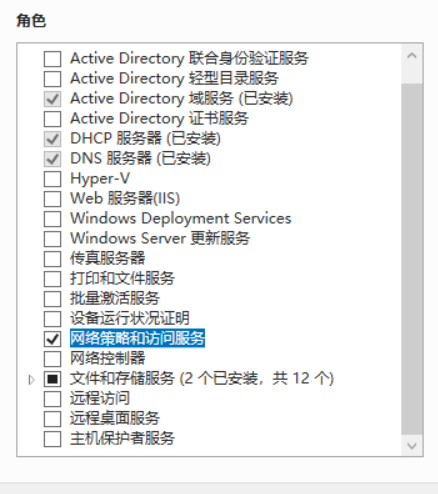
\includegraphics[width=0.65\textwidth]{img/26.png}
    \caption{安装网络策略和访问服务角色}
\end{figure}

完成安装后，在网络策略服务器控制台中创建 RADIUS 客户端。由于本实验中 VPN 服务与 RADIUS 服务部署在同一台服务器上，因此将 VPN 服务器作为 RADIUS 客户端添加到 NPS 中。实验中设置客户端名称为 \texttt{vpn-server}，客户端地址为 \texttt{192.168.126.10}，并手动配置共享机密，以便后续 VPN 服务器与 RADIUS 服务器之间能够进行一致的身份认证。相关配置如图所示。

\begin{figure}[H]
    \centering
    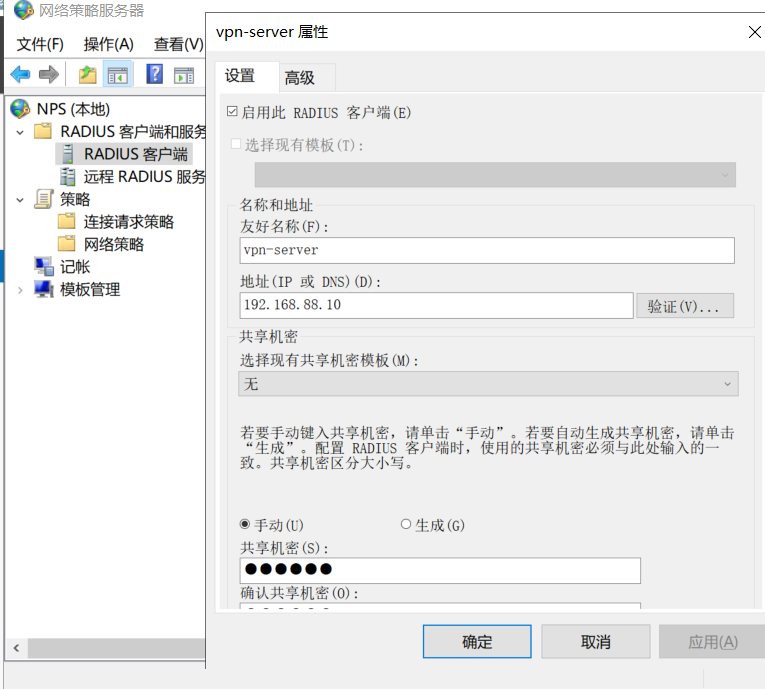
\includegraphics[width=0.62\textwidth]{img/27.png}
    \caption{配置 RADIUS 客户端}
\end{figure}

随后，在 NPS 中新建网络策略，用于控制远程 VPN 用户的访问权限。实验中将策略名称设置为“vpn访问策略”，网络访问服务器类型选择为“远程访问服务器（VPN 拨号）”。该策略用于处理来自 VPN 服务器的接入请求，并决定用户是否允许通过 RADIUS 认证接入内部网络。相关步骤如图所示。

\begin{figure}[H]
    \centering
    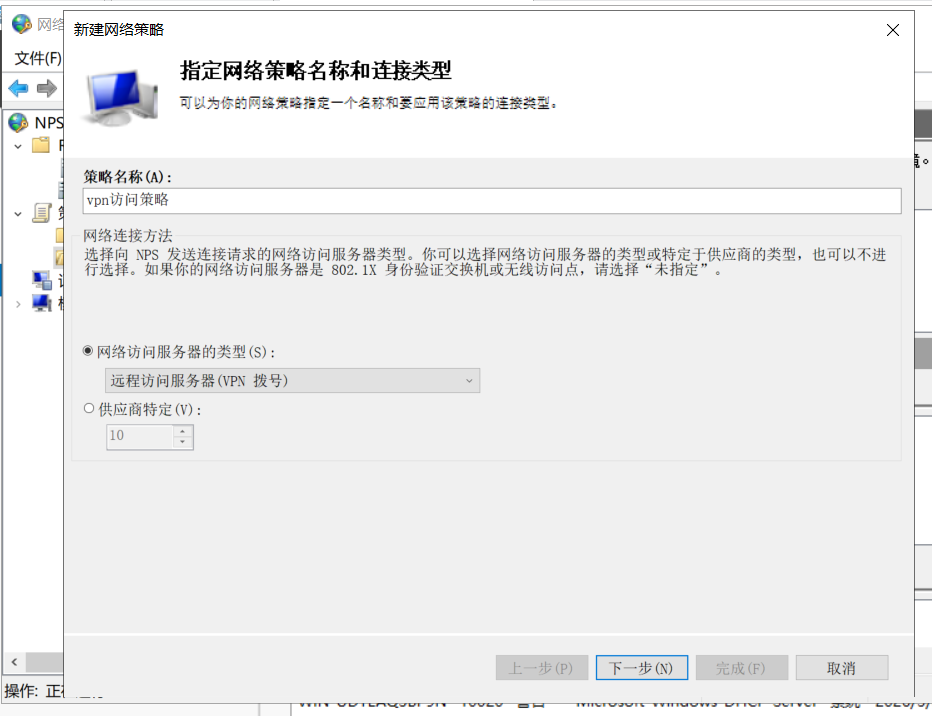
\includegraphics[width=0.72\textwidth]{img/28.png}
    \caption{新建 VPN 访问网络策略}
\end{figure}

在策略条件设置中，选择 \texttt{Windows 组} 作为认证条件，并将 \texttt{RADIUS\textbackslash Domain Users} 组加入策略匹配范围。这样，属于域用户组的用户即可在满足认证条件时通过该策略完成远程接入认证。相关设置如图所示。

\begin{figure}[H]
    \centering
    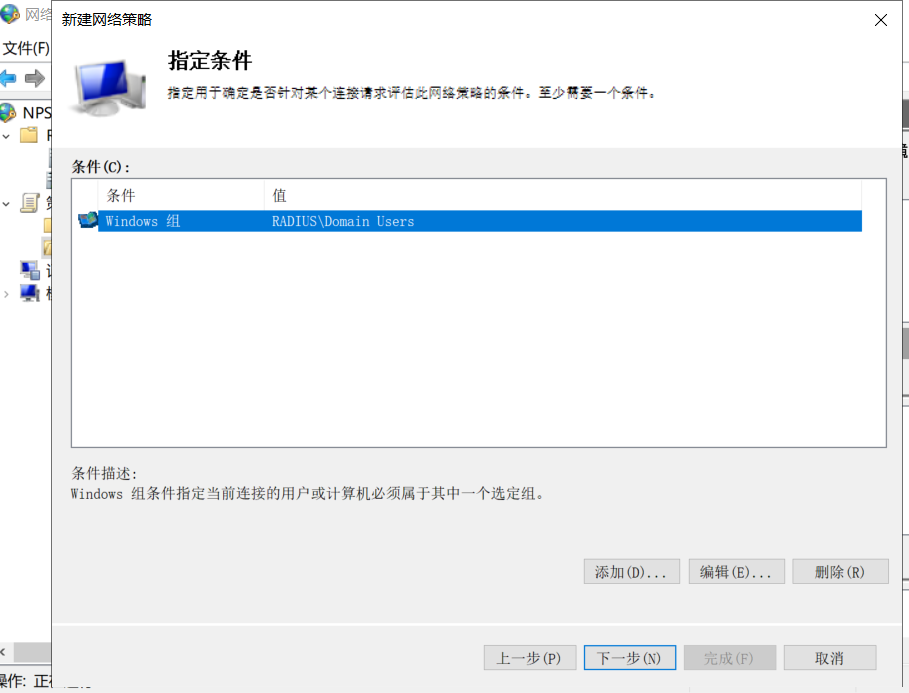
\includegraphics[width=0.72\textwidth]{img/29.png}
    \caption{配置网络策略条件}
\end{figure}

在网络策略属性中，启用该策略，并将访问权限设置为“授予访问权限”。这样，当用户的连接请求与该策略匹配时，NPS 将允许其通过身份验证并继续建立 VPN 连接。相关配置结果如图所示。

\begin{figure}[H]
    \centering
    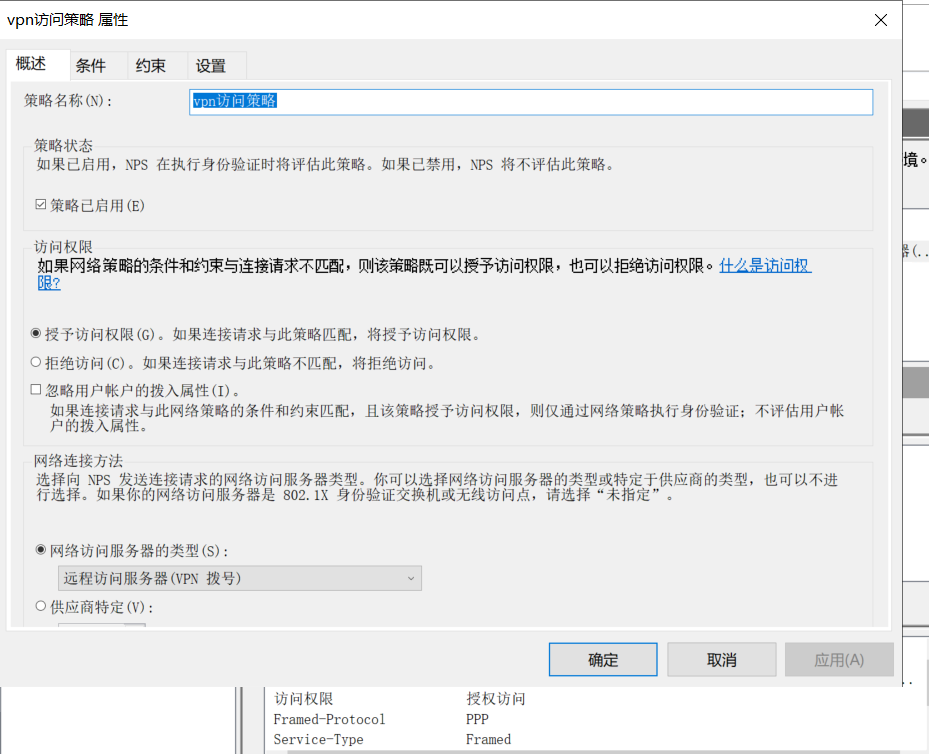
\includegraphics[width=0.72\textwidth]{img/30.png}
    \caption{配置网络策略访问权限}
\end{figure}

根据实验要求，远程访问用户需要使用“姓名+学号”的形式创建。因此，在“Active Directory 用户和计算机”中创建新的域用户，并将用户名设置为符合要求的格式。实验中创建的用户登录名为 \texttt{llb2023080904007@radius.local}，用户创建完成后即可作为后续 VPN 远程接入测试账号使用。相关过程如图所示。

\begin{figure}[H]
    \centering
    \begin{minipage}{0.48\textwidth}
        \centering
        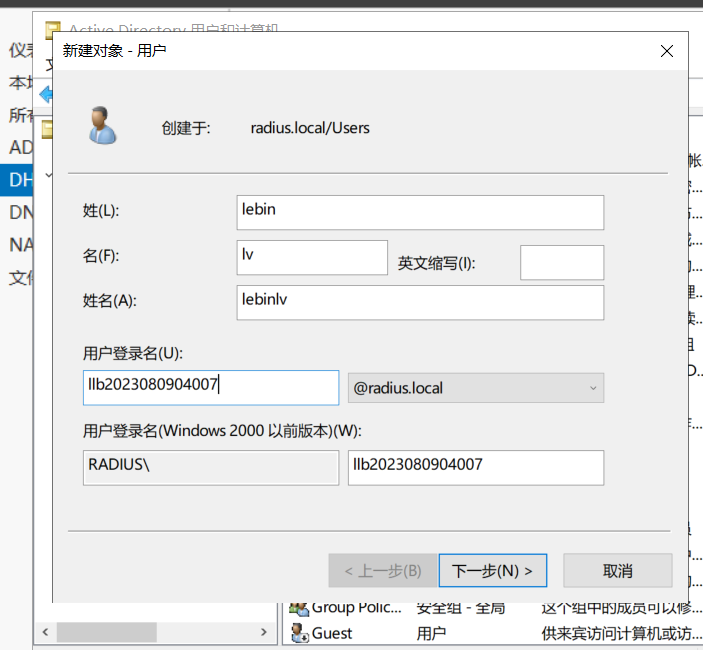
\includegraphics[width=\textwidth]{img/31.png}
    \end{minipage}
    \hfill
    \begin{minipage}{0.48\textwidth}
        \centering
        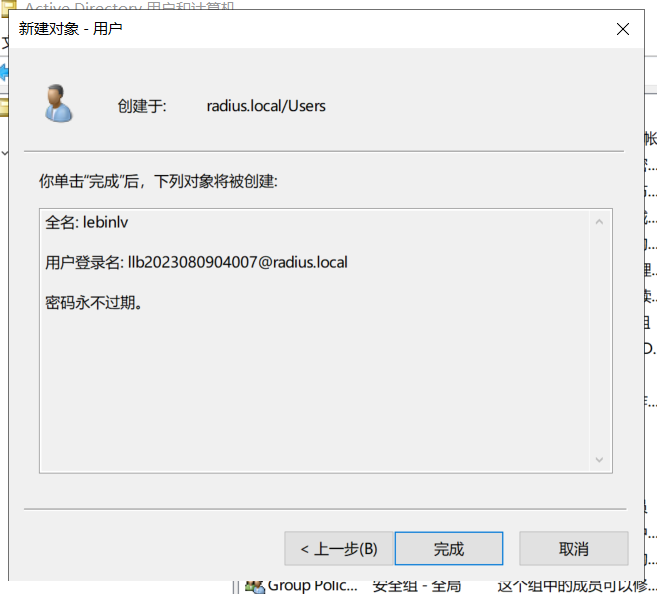
\includegraphics[width=\textwidth]{img/32.png}
    \end{minipage}
    \caption{创建符合要求的远程访问用户}
\end{figure}






\subsection*{5. 配置VPN服务器}

在完成域控制器、DNS、DHCP 以及 RADIUS 认证环境配置后，需要继续在 Windows Server 2022 上配置 VPN 服务器，使远程客户端能够通过外部网络接入内部网络。实验中通过安装“远程访问”角色，并启用“DirectAccess 和 VPN（RAS）”以及“路由”角色服务，为后续 VPN 远程接入提供基础支持。相关安装过程如图所示。

\begin{figure}[H]
    \centering
    \begin{minipage}{0.48\textwidth}
        \centering
        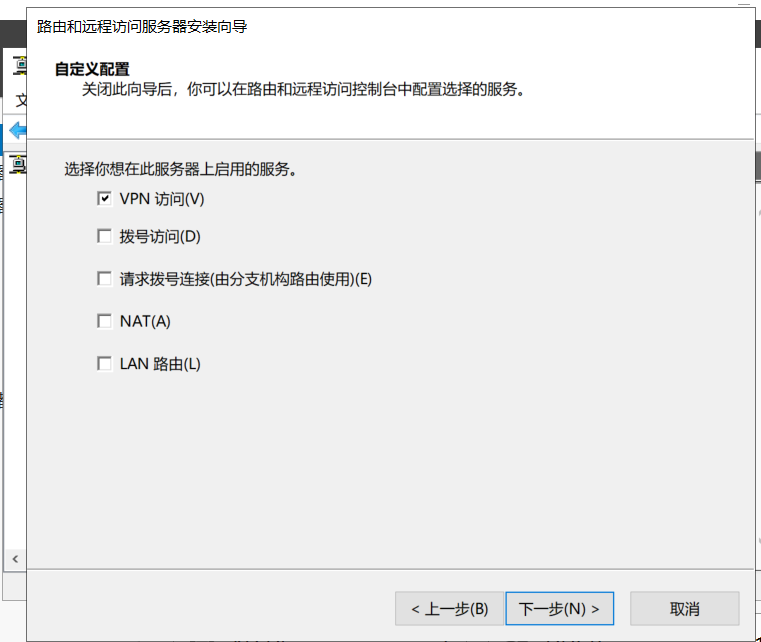
\includegraphics[width=\textwidth]{img/33.png}
    \end{minipage}
    \hfill
    \begin{minipage}{0.48\textwidth}
        \centering
        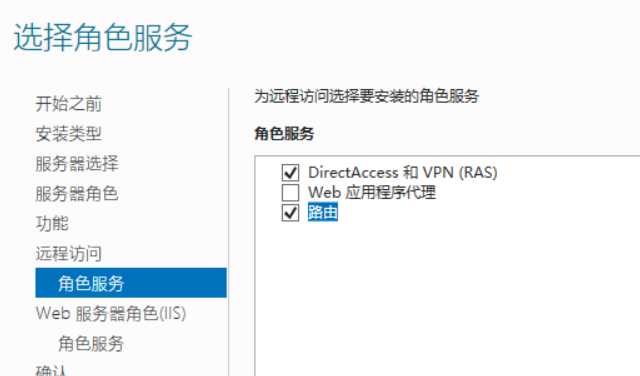
\includegraphics[width=\textwidth]{img/34.png}
    \end{minipage}
    \caption{安装远程访问角色及其角色服务}
\end{figure}

完成远程访问角色安装后，在“路由和远程访问”控制台中对服务器进行配置。实验中采用“自定义配置”方式，并在启用服务时勾选“VPN 访问”，使服务器能够接收远程客户端发起的 VPN 连接请求。相关配置过程如图所示。

\begin{figure}[H]
    \centering
    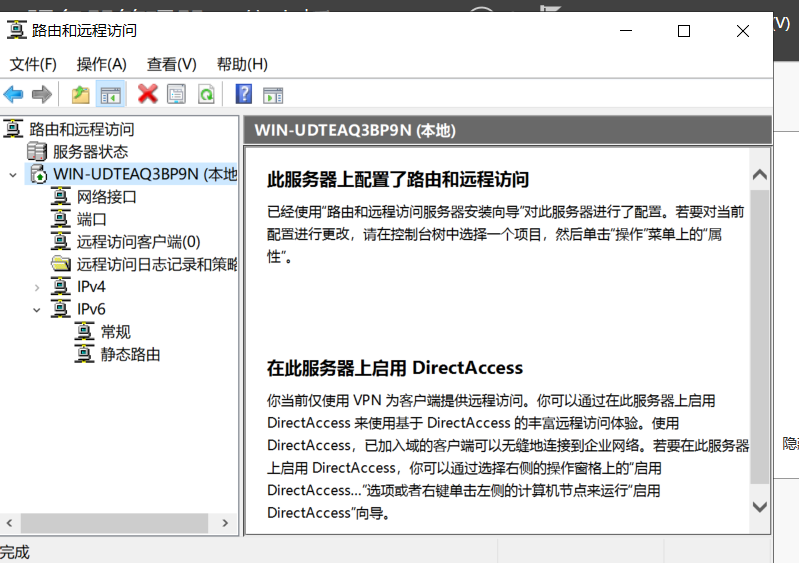
\includegraphics[width=0.68\textwidth]{img/35.png}
    \caption{在路由和远程访问服务中启用 VPN 访问}
\end{figure}

配置完成并启动服务后，服务器即进入“路由和远程访问”运行状态。此时服务器已经具备作为 VPN 接入服务器的基本能力，能够接收远程客户端的连接请求，并结合前面配置好的网络策略服务器（NPS）完成用户身份认证。由于本实验已部署网络策略服务器，远程访问认证将由 NPS 和网络策略共同处理，从而实现基于 RADIUS 的集中认证方式。配置完成后的控制台界面如图所示。

\begin{figure}[H]
    \centering
    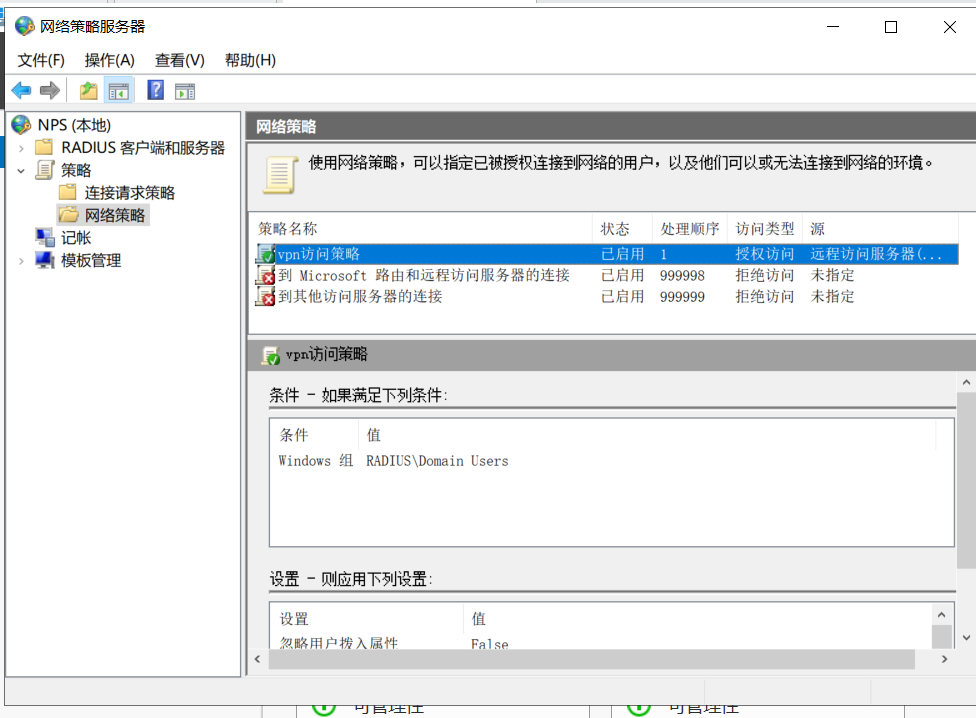
\includegraphics[width=0.78\textwidth]{img/36.png}
    \caption{VPN 服务器配置完成后的路由和远程访问界面}
\end{figure}

通过上述配置，Windows Server 2022 已成功启用 VPN 访问服务，为后续远程客户端创建 VPN 连接、使用“姓名+学号”账号进行认证登录，以及在 VPN 控制台中显示远程客户端连接状态奠定了基础。


\subsection*{6. 配置远程客户端与测试客户端连接}

在完成 VPN 服务器、RADIUS 认证服务以及远程访问用户配置后，需要在客户端主机上创建 VPN 连接，并使用前面创建的“姓名+学号”格式账号进行远程接入测试。实验中，首先在客户端测试其与 VPN 服务器外网地址 \texttt{192.168.126.10} 的连通性。测试结果表明，客户端能够正常与服务器通信，为后续建立 VPN 连接提供了网络基础。

\begin{figure}[H]
    \centering
    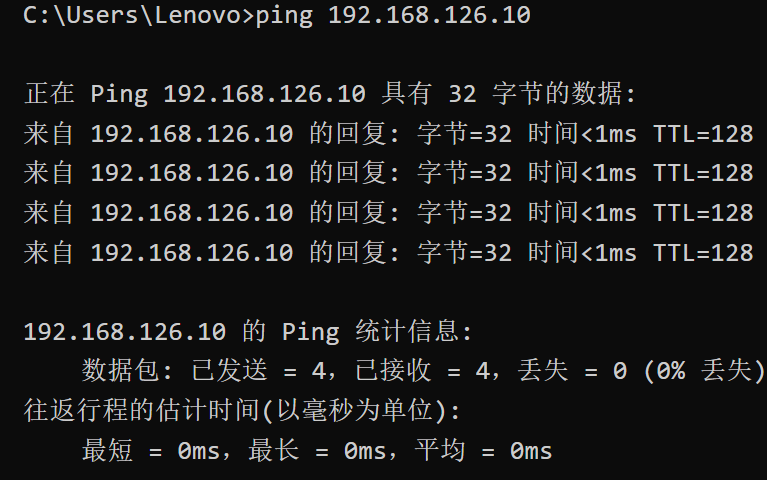
\includegraphics[width=0.72\textwidth]{img/37.png}
    \caption{客户端测试与 VPN 服务器的网络连通性}
\end{figure}

随后，在客户端“网络和共享中心”中创建新的 VPN 连接，服务器地址填写为 \texttt{192.168.126.10}，连接名称设置为 \texttt{radius-vpn}。在连接属性中，将 VPN 类型固定设置为 \texttt{PPTP}，以保证与服务器端配置一致。相关配置过程如图所示。

\begin{figure}[H]
    \centering
    \includegraphics[width=0.72\textwidth]{img/38.png}
    \caption{在客户端创建 VPN 连接}
\end{figure}

创建完成后，使用前面在域控制器中创建的远程访问账号进行登录。实验中采用“姓名+学号”格式的用户作为远程客户端登录账号，输入对应密码后发起连接请求。相关登录过程如图所示。

\begin{figure}[H]
    \centering
    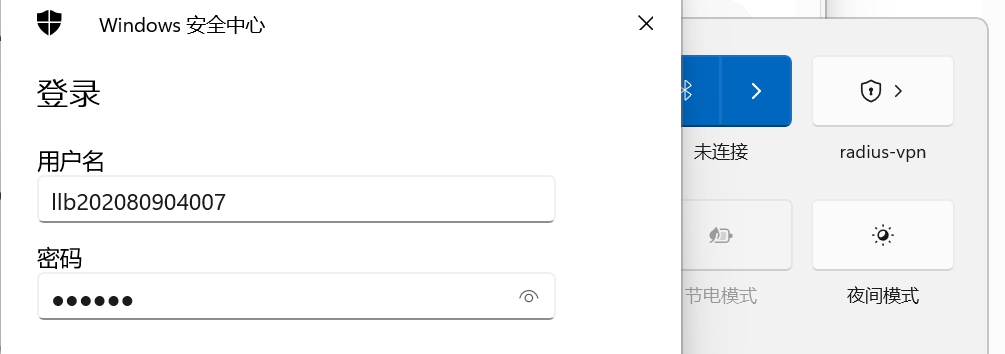
\includegraphics[width=0.56\textwidth]{img/39.png}
    \caption{使用远程访问用户账号进行 VPN 登录}
\end{figure}

当客户端连接成功后，系统显示 \texttt{radius-vpn} 已处于“已连接”状态，说明远程客户端已经成功建立 VPN 连接，能够通过该连接访问服务器提供的远程接入服务。相关结果如图所示。

\begin{figure}[H]
    \centering
    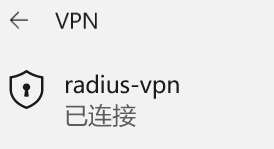
\includegraphics[width=0.42\textwidth]{img/40.png}
    \caption{客户端成功建立 VPN 连接}
\end{figure}

与此同时，在服务器端“路由和远程访问”控制台中，可以看到远程访问客户端列表中已经显示当前接入用户，说明客户端的连接请求已经被 VPN 服务器正确接收并建立会话。这表明远程客户端接入测试成功，VPN 服务器能够正常显示在线远程用户。相关结果如图所示。

\begin{figure}[H]
    \centering
  
    \begin{minipage}{0.48\textwidth}
        \centering
        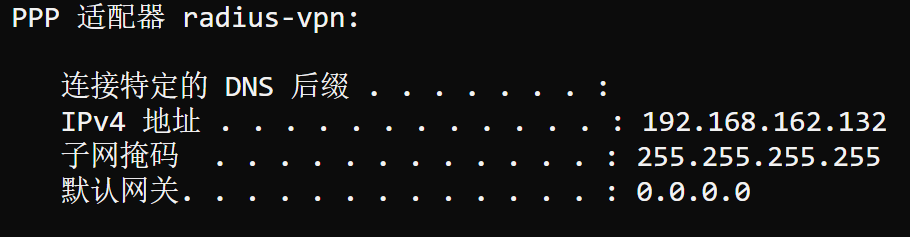
\includegraphics[width=\textwidth]{img/41.png}
    \end{minipage}
    \hfill
    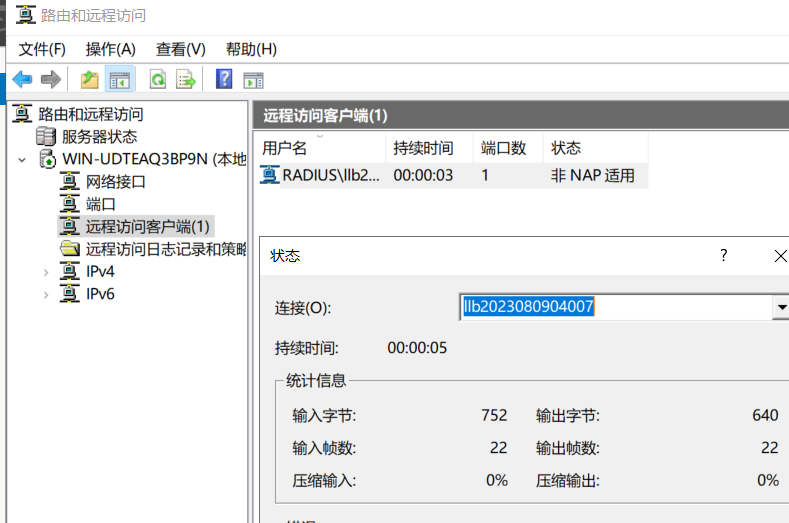
\includegraphics[width=0.78\textwidth]{img/42.png}
    \caption{服务器端显示远程客户端连接状态与在VPN中显示远程客户}
\end{figure}


\subsection*{补充实验：TCP端口扫描程序设计与测试}

根据实验要求，编写了一个基于 TCP Connect 扫描原理的主机端口扫描程序。程序能够由用户输入目标主机 IP 地址以及端口范围，对指定范围内的端口逐一进行连接测试，并输出各端口的状态（开放或关闭），从而判断目标主机中常见服务端口的开放情况。

\subsubsection*{（1）实验原理}

TCP 端口扫描的基本原理是：程序首先调用 \texttt{socket()} 函数创建流式套接字，其中 \texttt{SOCK\_STREAM} 表示使用 TCP 协议；然后调用 \texttt{connect()} 函数尝试与目标主机的指定端口建立连接。若连接成功，则说明该端口处于开放状态；若连接失败，则说明该端口未开放或目标主机拒绝连接。通过对指定范围内端口逐一执行上述过程，即可得到目标主机各端口的开放情况。

\subsubsection*{（2）程序设计思路}

本实验中的端口扫描程序采用命令行方式实现，整体设计思路如下：

\begin{enumerate}
    \item 程序启动后，首先初始化 Winsock 网络环境；
    \item 由用户输入目标主机 IP 地址、起始端口和结束端口；
    \item 程序对端口范围进行循环遍历；
    \item 对每一个端口，创建 TCP 套接字，并尝试与目标主机对应端口建立连接；
    \item 若连接成功，则输出“端口开放”；若连接失败，则输出“端口关闭”；
    \item 全部端口扫描完成后，输出扫描结束信息并释放网络资源。
\end{enumerate}

其核心流程可以概括为：  
\textbf{输入目标 IP 和端口范围 $\rightarrow$ 创建套接字 $\rightarrow$ 调用 connect() 连接目标端口 $\rightarrow$ 判断连接结果 $\rightarrow$ 输出端口状态。}

\subsubsection*{（3）程序核心代码}

程序中最关键的部分是端口开放检测函数 \texttt{isPortOpen()}，其主要思想是：创建 TCP 套接字后，向目标主机指定端口发起连接请求，并根据返回结果判断端口状态。核心代码如下：

\begin{verbatim}
bool isPortOpen(const string& ip, int port, int timeoutMs = 1000) {
    SOCKET sock = socket(AF_INET, SOCK_STREAM, IPPROTO_TCP);
    if (sock == INVALID_SOCKET) {
        return false;
    }

    u_long mode = 1;
    ioctlsocket(sock, FIONBIO, &mode);

    sockaddr_in targetAddr{};
    targetAddr.sin_family = AF_INET;
    targetAddr.sin_port = htons(port);

    if (inet_pton(AF_INET, ip.c_str(), &targetAddr.sin_addr) <= 0) {
        closesocket(sock);
        return false;
    }

    int result = connect(sock, (sockaddr*)&targetAddr, sizeof(targetAddr));

    if (result == SOCKET_ERROR) {
        int err = WSAGetLastError();
        if (err != WSAEWOULDBLOCK && err != WSAEINPROGRESS && err != WSAEINVAL) {
            closesocket(sock);
            return false;
        }
    }

    fd_set writeSet;
    FD_ZERO(&writeSet);
    FD_SET(sock, &writeSet);

    timeval timeout{};
    timeout.tv_sec = timeoutMs / 1000;
    timeout.tv_usec = (timeoutMs % 1000) * 1000;

    result = select(0, NULL, &writeSet, NULL, &timeout);

    if (result > 0 && FD_ISSET(sock, &writeSet)) {
        int so_error = 0;
        int len = sizeof(so_error);
        getsockopt(sock, SOL_SOCKET, SO_ERROR, (char*)&so_error, &len);
        closesocket(sock);
        return so_error == 0;
    }

    closesocket(sock);
    return false;
}
\end{verbatim}

上述函数通过创建非阻塞套接字，并结合 \texttt{select()} 设置超时等待机制，在避免程序长时间阻塞的同时，提高了端口扫描过程的稳定性。

\subsubsection*{（4）程序完整代码}

详细见附录1。

\subsubsection*{（5）测试结果}

在实验测试中，首先以服务器主机 \texttt{192.168.162.10} 为目标，对端口范围 \texttt{75$\sim$85} 进行扫描。结果显示，在该端口范围内，仅 \texttt{80} 号端口处于开放状态，其余端口均为关闭状态。这说明目标主机上对应的 Web 服务端口处于监听状态，程序能够正确识别开放端口与关闭端口。测试结果如图所示。

\begin{figure}[H]
    \centering
    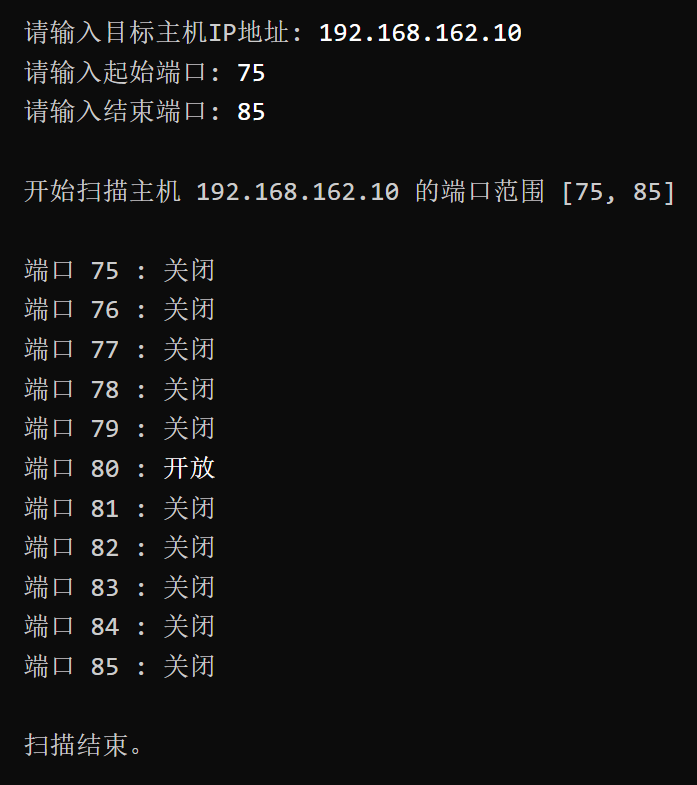
\includegraphics[width=0.78\textwidth]{img/43.png}
    \caption{扫描主机 \texttt{192.168.162.10} 的 \texttt{75$\sim$85} 端口结果}
\end{figure}

随后，继续对同一目标主机的 \texttt{443} 端口进行单端口扫描。结果显示，\texttt{443} 号端口为开放状态，说明目标主机上的 HTTPS/SSL 服务端口处于开启状态。该结果与实验环境中 SSL 服务的配置情况相符，进一步验证了程序对单个目标端口开放状态的检测能力。测试结果如图所示。

\begin{figure}[H]
    \centering
    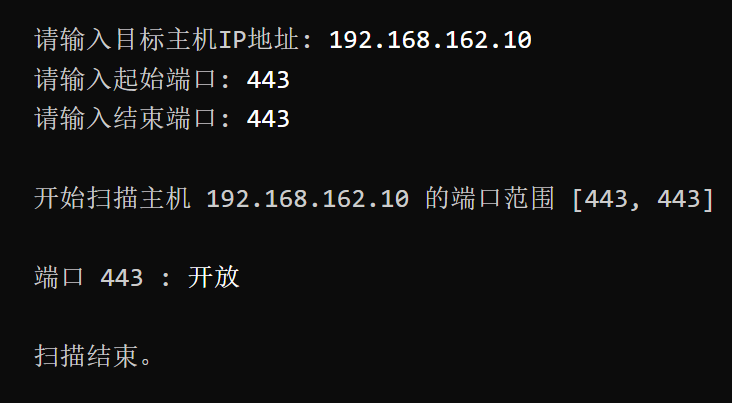
\includegraphics[width=0.78\textwidth]{img/44.png}
    \caption{扫描主机 \texttt{192.168.162.10} 的 \texttt{443} 端口结果}
\end{figure}

此外，为了验证程序对端口范围扫描功能的实现情况，又以本地主机 \texttt{127.0.0.1} 为目标，对 \texttt{1$\sim$128} 范围内的端口进行了扫描。扫描结果中可以看到程序能够逐一输出各端口的状态信息，体现了其对连续端口范围进行自动扫描的能力。虽然结果中大多数端口处于关闭状态，但该测试说明程序已经能够按照设定范围逐端口完成检测并输出结果。测试结果如图所示。

\begin{figure}[H]
    \centering
    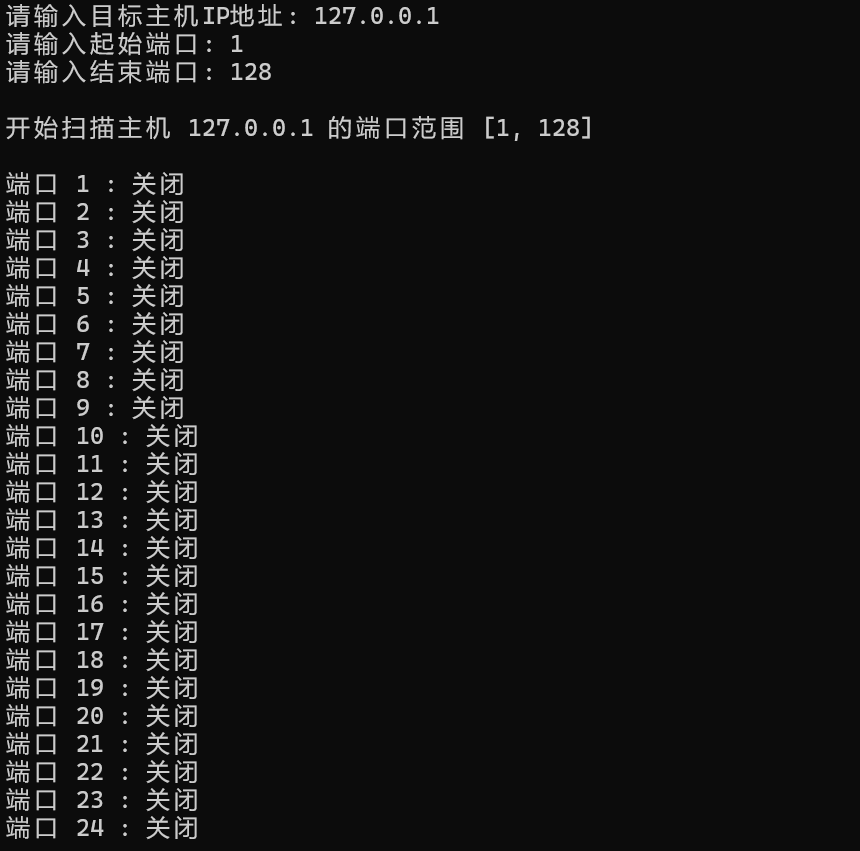
\includegraphics[width=0.72\textwidth]{img/45.png}
    \caption{扫描本地主机 \texttt{127.0.0.1} 的 \texttt{1$\sim$128} 端口结果}
\end{figure}

\subsubsection*{（6）结果分析}

综合以上测试结果可以看出，该 TCP 端口扫描程序能够正确实现对目标主机指定端口及端口范围的扫描，并根据连接结果判断端口的开放或关闭状态。程序不仅能够识别常见的 Web 服务端口 \texttt{80} 和 SSL 服务端口 \texttt{443} 的开放情况，还能够完成对多个连续端口的范围扫描，说明其基本满足实验要求。

通过本补充实验，进一步加深了对 TCP 套接字、\texttt{connect()} 连接机制以及主机端口状态检测原理的理解，也验证了基于套接字的 TCP Connect 扫描方法在主机服务探测中的实际应用。


{\heiti\zihao{4} 八、实验结论、心得体会和改进建议：}

通过本次 Radius 综合实验，成功在 Windows Server 2022 环境下完成了域控制器、DNS 服务器、DHCP 服务器、网络策略服务器（NPS）、VPN 服务器等服务的综合配置，搭建了一个较完整的远程接入认证环境。实验中，远程客户端能够通过配置好的 VPN 连接访问服务器，并使用“姓名+学号”格式创建的域用户账号完成身份认证；服务器端“路由和远程访问”控制台中能够显示远程访问客户端信息，客户端也成功获得了内部网络地址，说明 VPN 服务与 Radius 认证过程已经能够协同工作，基本达到了实验要求。

通过本实验，加深了对 Radius 协议、AAA 机制以及 VPN 远程接入原理的理解。对 Windows Server 中域控制器、DNS、DHCP、NPS 和路由与远程访问服务之间的关系有了更加直观的认识，也进一步掌握了基于 Windows Server 的远程接入认证环境搭建方法。在实验过程中，还通过补充实验编写了 TCP 端口扫描程序，进一步理解了套接字编程、TCP Connect 扫描原理以及网络服务端口开放状态的检测方法。

在实验过程中，也遇到了一些问题，例如双网卡配置容易混淆、DHCP 授权和作用域配置需要仔细检查、NPS 与 RRAS 的认证关系不够直观，以及客户端连接后内部地址分配的调试较为繁琐。这些问题说明在综合网络实验中，不同服务之间的关联性很强，一个环节配置不正确就可能影响整个实验结果。因此，在后续实验中需要更加注意网络环境规划、地址分配设计以及服务之间的依赖关系。

针对本实验，还可以从以下几个方面进行改进：一是进一步优化网络拓扑设计，使外网和内网的逻辑更加清晰，减少地址分配和接口绑定时的混淆；二是对 NPS 的连接请求策略、网络策略以及 RRAS 的联动机制进行更深入分析，以便更加准确地定位认证失败的原因；三是对补充实验中的端口扫描程序进行改进，例如增加多线程扫描、扫描超时设置优化以及结果输出格式优化，从而提高程序运行效率和实用性。

总体来看，本实验不仅完成了 Windows Server 下 VPN 与 Radius 综合认证环境的搭建，还锻炼了对网络服务综合配置、问题排查和实验分析的能力，具有较强的实践意义。

{\heiti\zihao{4} 附录1}


\begin{verbatim}
#include <iostream>
#include <string>
#include <winsock2.h>
#include <ws2tcpip.h>

#pragma comment(lib, "ws2_32.lib")

using namespace std;

bool isPortOpen(const string& ip, int port, int timeoutMs = 1000) {
    SOCKET sock = socket(AF_INET, SOCK_STREAM, IPPROTO_TCP);
    if (sock == INVALID_SOCKET) {
        return false;
    }

    u_long mode = 1;
    ioctlsocket(sock, FIONBIO, &mode);

    sockaddr_in targetAddr{};
    targetAddr.sin_family = AF_INET;
    targetAddr.sin_port = htons(port);

    if (inet_pton(AF_INET, ip.c_str(), &targetAddr.sin_addr) <= 0) {
        closesocket(sock);
        return false;
    }

    int result = connect(sock, (sockaddr*)&targetAddr, sizeof(targetAddr));

    if (result == SOCKET_ERROR) {
        int err = WSAGetLastError();
        if (err != WSAEWOULDBLOCK && err != WSAEINPROGRESS && err != WSAEINVAL) {
            closesocket(sock);
            return false;
        }
    }

    fd_set writeSet;
    FD_ZERO(&writeSet);
    FD_SET(sock, &writeSet);

    timeval timeout{};
    timeout.tv_sec = timeoutMs / 1000;
    timeout.tv_usec = (timeoutMs % 1000) * 1000;

    result = select(0, NULL, &writeSet, NULL, &timeout);

    if (result > 0 && FD_ISSET(sock, &writeSet)) {
        int so_error = 0;
        int len = sizeof(so_error);
        getsockopt(sock, SOL_SOCKET, SO_ERROR, (char*)&so_error, &len);
        closesocket(sock);
        return so_error == 0;
    }

    closesocket(sock);
    return false;
}

int main() {
    WSADATA wsaData;
    int wsaResult = WSAStartup(MAKEWORD(2, 2), &wsaData);
    if (wsaResult != 0) {
        cerr << "Winsock 初始化失败，错误码: " << wsaResult << endl;
        return 1;
    }

    string targetIp;
    int startPort, endPort;

    cout << "请输入目标主机IP地址: ";
    cin >> targetIp;

    cout << "请输入起始端口: ";
    cin >> startPort;

    cout << "请输入结束端口: ";
    cin >> endPort;

    if (startPort < 1 || endPort > 65535 || startPort > endPort) {
        cerr << "端口范围输入不合法！" << endl;
        WSACleanup();
        return 1;
    }

    cout << "\n开始扫描主机 " << targetIp
         << " 的端口范围 [" << startPort << ", " << endPort << "]\n" << endl;

    for (int port = startPort; port <= endPort; ++port) {
        bool open = isPortOpen(targetIp, port);
        if (open) {
            cout << "端口 " << port << " : 开放" << endl;
        } else {
            cout << "端口 " << port << " : 关闭" << endl;
        }
    }

    cout << "\n扫描结束。" << endl;

    WSACleanup();
    return 0;
}
\end{verbatim}
\end{document}